% App. D figure: the time-centred coupling score on one real window.
\begin{tikzpicture}[x=1cm,y=1cm]
% ---------------------------------------------------------------- embeddings
\node[inner sep=0,anchor=west] (e) at (0,1.35) {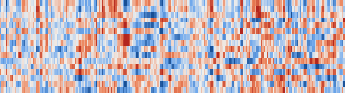
\includegraphics[width=3.2cm,height=0.8cm]{figures/net_emb_e.pdf}};
\node[inner sep=0,anchor=west] (a1) at (0,0) {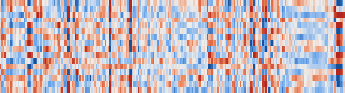
\includegraphics[width=3.2cm,height=0.8cm]{figures/net_emb_a1.pdf}};
\node[inner sep=0,anchor=west] (a2) at (0,-1.1) {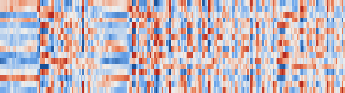
\includegraphics[width=3.2cm,height=0.8cm]{figures/net_emb_a2.pdf}};
\draw[cfN,line width=0.8pt] (e.south west) rectangle (e.north east);
\draw[cfA,line width=0.8pt] (a1.south west) rectangle (a1.north east);
\draw[cfA!55,line width=0.8pt] (a2.south west) rectangle (a2.north east);
\node[font=\scriptsize,text=cfN,anchor=south west,inner sep=1pt] at (e.north west) {EEG embedding $e$ ($16\times L$)};
\node[font=\scriptsize,text=cfA,anchor=south west,inner sep=1pt] at (a1.north west) {$\hat{a}_1$, attended talker};
\node[font=\scriptsize,text=cfA!80!black,anchor=south west,inner sep=1pt] at (a2.north west) {$\hat{a}_2$, competing talker};
\node[note,anchor=north west] at ($(a2.south west)+(0,-0.05)$) {rows: 16 dimensions; columns: 5\,s};

% ---------------------------------------------------------------- operations
\node[nbw={cfC}{2.25}] (cz) at (4.75,0.15) {centre and\\normalise each\\dimension over $t$};
\draw[ar=cfN] (e.east) -- ++(0.2,0) |- ([yshift=0.18cm]cz.west);
\draw[ar=cfA] (a1.east) -- ([yshift=-0.0cm]cz.west);
\draw[ar=cfA!55] (a2.east) -- ++(0.2,0) |- ([yshift=-0.18cm]cz.west);
\node[nbw={cfC}{2.35}] (rho) at (7.45,0.15)
  {$r_{k,d}=\mathrm{corr}_t\big(e_d,\hat a_{k,d}\big)$\\[1pt]one per candidate\\and dimension};
\draw[ar=cfC] (cz) -- (rho);
\node[inner sep=0,anchor=north] (bars) at (7.45,-0.75)
  {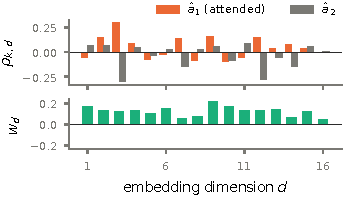
\includegraphics[width=3.1cm]{figures/net_emb_corr.pdf}};
\node[nbw={cfC}{2.35}] (sum) at (10.35,0.15)
  {$s_k=\frac1\tau\sum_d \omega_d\,r_{k,d}$\\[1pt]learned $\omega_d$ (bars),\\$\tau=\netTau$};
\draw[ar=cfC] (rho) -- (sum);
\node[nbw={cfC}{2.1}] (cen) at (13.0,0.15)
  {centre over $k$\\$s_k-\tfrac1K\sum_j s_j$};
\draw[ar=cfC] (sum) -- (cen);
\node[nbw={cfC}{1.85},line width=0.9pt] (out) at (13.1,-1.45)
  {$s_1=\netSOne$\\$s_2=\netSTwo$\\[1pt]$\hat y=1$ \checkmark};
\draw[ar=cfC] (cen) -- (out) node[arl,midway,right=1pt] {this window};

% ---------------------------------------------------------------- null inset
\node[draw=cfG,fill=cfG!6,rounded corners=2pt,line width=0.6pt,anchor=north west,
      text width=2.75cm,font=\tiny,align=left,inner sep=3pt] (null) at (9.2,-0.95)
  {\raggedright\textbf{\scriptsize Null case.} If $e$ is constant in time, centring makes it
   zero, every $r_{k,d}=0$ and every $s_k=0$: a tie, counted as an error. The audio
   embeddings alone cannot move the decision (Prop.~\ref{prop:null}).};
\end{tikzpicture}
